
%% bare_jrnl.tex
%% V1.3
%% 2007/01/11
%% by Michael Shell
%% see http://www.michaelshell.org/
%% for current contact information.
%%
%% This is a skeleton file demonstrating the use of IEEEtran.cls
%% (requires IEEEtran.cls version 1.7 or later) with an IEEE journal paper.
%%
%% Support sites:
%% http://www.michaelshell.org/tex/ieeetran/
%% http://www.ctan.org/tex-archive/macros/latex/contrib/IEEEtran/
%% and
%% http://www.ieee.org/



% *** Authors should verify (and, if needed, correct) their LaTeX system  ***
% *** with the testflow diagnostic prior to trusting their LaTeX platform ***
% *** with production work. IEEE's font choices can trigger bugs that do  ***
% *** not appear when using other class files.                            ***
% The testflow support page is at:
% http://www.michaelshell.org/tex/testflow/


%%*************************************************************************
%% Legal Notice:
%% This code is offered as-is without any warranty either expressed or
%% implied; without even the implied warranty of MERCHANTABILITY or
%% FITNESS FOR A PARTICULAR PURPOSE! 
%% User assumes all risk.
%% In no event shall IEEE or any contributor to this code be liable for
%% any damages or losses, including, but not limited to, incidental,
%% consequential, or any other damages, resulting from the use or misuse
%% of any information contained here.
%%
%% All comments are the opinions of their respective authors and are not
%% necessarily endorsed by the IEEE.
%%
%% This work is distributed under the LaTeX Project Public License (LPPL)
%% ( http://www.latex-project.org/ ) version 1.3, and may be freely used,
%% distributed and modified. A copy of the LPPL, version 1.3, is included
%% in the base LaTeX documentation of all distributions of LaTeX released
%% 2003/12/01 or later.
%% Retain all contribution notices and credits.
%% ** Modified files should be clearly indicated as such, including  **
%% ** renaming them and changing author support contact information. **
%%
%% File list of work: IEEEtran.cls, IEEEtran_HOWTO.pdf, bare_adv.tex,
%%                    bare_conf.tex, bare_jrnl.tex, bare_jrnl_compsoc.tex
%%*************************************************************************

% Note that the a4paper option is mainly intended so that authors in
% countries using A4 can easily print to A4 and see how their papers will
% look in print - the typesetting of the document will not typically be
% affected with changes in paper size (but the bottom and side margins will).
% Use the testflow package mentioned above to verify correct handling of
% both paper sizes by the user's LaTeX system.
%
% Also note that the "draftcls" or "draftclsnofoot", not "draft", option
% should be used if it is desired that the figures are to be displayed in
% draft mode.
%
\documentclass[journal,twoside]{IEEEtran}
\usepackage{blindtext}
\usepackage{graphicx}
\usepackage{multirow}
\usepackage{amsmath}
\usepackage{acro}

\acsetup{first-style=short}
\DeclareAcronym{lcs}{
  short = LCS ,
  long  = Longest Common Subsequence ,
  class = abbrev
}
% Some very useful LaTeX packages include:
% (uncomment the ones you want to load)


% *** MISC UTILITY PACKAGES ***
%
%\usepackage{ifpdf}
% Heiko Oberdiek's ifpdf.sty is very useful if you need conditional
% compilation based on whether the output is pdf or dvi.
% usage:
% \ifpdf
%   % pdf code
% \else
%   % dvi code
% \fi
% The latest version of ifpdf.sty can be obtained from:
% http://www.ctan.org/tex-archive/macros/latex/contrib/oberdiek/
% Also, note that IEEEtran.cls V1.7 and later provides a builtin
% \ifCLASSINFOpdf conditional that works the same way.
% When switching from latex to pdflatex and vice-versa, the compiler may
% have to be run twice to clear warning/error messages.






% *** CITATION PACKAGES ***
%
%\usepackage{cite}
% cite.sty was written by Donald Arseneau
% V1.6 and later of IEEEtran pre-defines the format of the cite.sty package
% \cite{} output to follow that of IEEE. Loading the cite package will
% result in citation numbers being automatically sorted and properly
% "compressed/ranged". e.g., [1], [9], [2], [7], [5], [6] without using
% cite.sty will become [1], [2], [5]--[7], [9] using cite.sty. cite.sty's
% \cite will automatically add leading space, if needed. Use cite.sty's
% noadjust option (cite.sty V3.8 and later) if you want to turn this off.
% cite.sty is already installed on most LaTeX systems. Be sure and use
% version 4.0 (2003-05-27) and later if using hyperref.sty. cite.sty does
% not currently provide for hyperlinked citations.
% The latest version can be obtained at:
% http://www.ctan.org/tex-archive/macros/latex/contrib/cite/
% The documentation is contained in the cite.sty file itself.






% *** GRAPHICS RELATED PACKAGES ***
%
\ifCLASSINFOpdf
  % \usepackage[pdftex]{graphicx}
  % declare the path(s) where your graphic files are
  % \graphicspath{{../pdf/}{../jpeg/}}
  % and their extensions so you won't have to specify these with
  % every instance of \includegraphics
  % \DeclareGraphicsExtensions{.pdf,.jpeg,.png}
\else
  % or other class option (dvipsone, dvipdf, if not using dvips). graphicx
  % will default to the driver specified in the system graphics.cfg if no
  % driver is specified.
  % \usepackage[dvips]{graphicx}
  % declare the path(s) where your graphic files are
  % \graphicspath{{../eps/}}
  % and their extensions so you won't have to specify these with
  % every instance of \includegraphics
  % \DeclareGraphicsExtensions{.eps}
\fi
% graphicx was written by David Carlisle and Sebastian Rahtz. It is
% required if you want graphics, photos, etc. graphicx.sty is already
% installed on most LaTeX systems. The latest version and documentation can
% be obtained at: 
% http://www.ctan.org/tex-archive/macros/latex/required/graphics/
% Another good source of documentation is "Using Imported Graphics in
% LaTeX2e" by Keith Reckdahl which can be found as epslatex.ps or
% epslatex.pdf at: http://www.ctan.org/tex-archive/info/
%
% latex, and pdflatex in dvi mode, support graphics in encapsulated
% postscript (.eps) format. pdflatex in pdf mode supports graphics
% in .pdf, .jpeg, .png and .mps (metapost) formats. Users should ensure
% that all non-photo figures use a vector format (.eps, .pdf, .mps) and
% not a bitmapped formats (.jpeg, .png). IEEE frowns on bitmapped formats
% which can result in "jaggedy"/blurry rendering of lines and letters as
% well as large increases in file sizes.
%
% You can find documentation about the pdfTeX application at:
% http://www.tug.org/applications/pdftex





% *** MATH PACKAGES ***
%
%\usepackage[cmex10]{amsmath}
% A popular package from the American Mathematical Society that provides
% many useful and powerful commands for dealing with mathematics. If using
% it, be sure to load this package with the cmex10 option to ensure that
% only type 1 fonts will utilized at all point sizes. Without this option,
% it is possible that some math symbols, particularly those within
% footnotes, will be rendered in bitmap form which will result in a
% document that can not be IEEE Xplore compliant!
%
% Also, note that the amsmath package sets \interdisplaylinepenalty to 10000
% thus preventing page breaks from occurring within multiline equations. Use:
%\interdisplaylinepenalty=2500
% after loading amsmath to restore such page breaks as IEEEtran.cls normally
% does. amsmath.sty is already installed on most LaTeX systems. The latest
% version and documentation can be obtained at:
% http://www.ctan.org/tex-archive/macros/latex/required/amslatex/math/





% *** SPECIALIZED LIST PACKAGES ***
%
%\usepackage{algorithmic}
% algorithmic.sty was written by Peter Williams and Rogerio Brito.
% This package provides an algorithmic environment fo describing algorithms.
% You can use the algorithmic environment in-text or within a figure
% environment to provide for a floating algorithm. Do NOT use the algorithm
% floating environment provided by algorithm.sty (by the same authors) or
% algorithm2e.sty (by Christophe Fiorio) as IEEE does not use dedicated
% algorithm float types and packages that provide these will not provide
% correct IEEE style captions. The latest version and documentation of
% algorithmic.sty can be obtained at:
% http://www.ctan.org/tex-archive/macros/latex/contrib/algorithms/
% There is also a support site at:
% http://algorithms.berlios.de/index.html
% Also of interest may be the (relatively newer and more customizable)
% algorithmicx.sty package by Szasz Janos:
% http://www.ctan.org/tex-archive/macros/latex/contrib/algorithmicx/




% *** ALIGNMENT PACKAGES ***
%
%\usepackage{array}
% Frank Mittelbach's and David Carlisle's array.sty patches and improves
% the standard LaTeX2e array and tabular environments to provide better
% appearance and additional user controls. As the default LaTeX2e table
% generation code is lacking to the point of almost being broken with
% respect to the quality of the end results, all users are strongly
% advised to use an enhanced (at the very least that provided by array.sty)
% set of table tools. array.sty is already installed on most systems. The
% latest version and documentation can be obtained at:
% http://www.ctan.org/tex-archive/macros/latex/required/tools/


%\usepackage{mdwmath}
%\usepackage{mdwtab}
% Also highly recommended is Mark Wooding's extremely powerful MDW tools,
% especially mdwmath.sty and mdwtab.sty which are used to format equations
% and tables, respectively. The MDWtools set is already installed on most
% LaTeX systems. The lastest version and documentation is available at:
% http://www.ctan.org/tex-archive/macros/latex/contrib/mdwtools/


% IEEEtran contains the IEEEeqnarray family of commands that can be used to
% generate multiline equations as well as matrices, tables, etc., of high
% quality.


%\usepackage{eqparbox}
% Also of notable interest is Scott Pakin's eqparbox package for creating
% (automatically sized) equal width boxes - aka "natural width parboxes".
% Available at:
% http://www.ctan.org/tex-archive/macros/latex/contrib/eqparbox/





% *** SUBFIGURE PACKAGES ***
%\usepackage[tight,footnotesize]{subfigure}
% subfigure.sty was written by Steven Douglas Cochran. This package makes it
% easy to put subfigures in your figures. e.g., "Figure 1a and 1b". For IEEE
% work, it is a good idea to load it with the tight package option to reduce
% the amount of white space around the subfigures. subfigure.sty is already
% installed on most LaTeX systems. The latest version and documentation can
% be obtained at:
% http://www.ctan.org/tex-archive/obsolete/macros/latex/contrib/subfigure/
% subfigure.sty has been superceeded by subfig.sty.



%\usepackage[caption=false]{caption}
%\usepackage[font=footnotesize]{subfig}
% subfig.sty, also written by Steven Douglas Cochran, is the modern
% replacement for subfigure.sty. However, subfig.sty requires and
% automatically loads Axel Sommerfeldt's caption.sty which will override
% IEEEtran.cls handling of captions and this will result in nonIEEE style
% figure/table captions. To prevent this problem, be sure and preload
% caption.sty with its "caption=false" package option. This is will preserve
% IEEEtran.cls handing of captions. Version 1.3 (2005/06/28) and later 
% (recommended due to many improvements over 1.2) of subfig.sty supports
% the caption=false option directly:
%\usepackage[caption=false,font=footnotesize]{subfig}
%
% The latest version and documentation can be obtained at:
% http://www.ctan.org/tex-archive/macros/latex/contrib/subfig/
% The latest version and documentation of caption.sty can be obtained at:
% http://www.ctan.org/tex-archive/macros/latex/contrib/caption/




% *** FLOAT PACKAGES ***
%
%\usepackage{fixltx2e}
% fixltx2e, the successor to the earlier fix2col.sty, was written by
% Frank Mittelbach and David Carlisle. This package corrects a few problems
% in the LaTeX2e kernel, the most notable of which is that in current
% LaTeX2e releases, the ordering of single and double column floats is not
% guaranteed to be preserved. Thus, an unpatched LaTeX2e can allow a
% single column figure to be placed prior to an earlier double column
% figure. The latest version and documentation can be found at:
% http://www.ctan.org/tex-archive/macros/latex/base/



%\usepackage{stfloats}
% stfloats.sty was written by Sigitas Tolusis. This package gives LaTeX2e
% the ability to do double column floats at the bottom of the page as well
% as the top. (e.g., "\begin{figure*}[!b]" is not normally possible in
% LaTeX2e). It also provides a command:
%\fnbelowfloat
% to enable the placement of footnotes below bottom floats (the standard
% LaTeX2e kernel puts them above bottom floats). This is an invasive package
% which rewrites many portions of the LaTeX2e float routines. It may not work
% with other packages that modify the LaTeX2e float routines. The latest
% version and documentation can be obtained at:
% http://www.ctan.org/tex-archive/macros/latex/contrib/sttools/
% Documentation is contained in the stfloats.sty comments as well as in the
% presfull.pdf file. Do not use the stfloats baselinefloat ability as IEEE
% does not allow \baselineskip to stretch. Authors submitting work to the
% IEEE should note that IEEE rarely uses double column equations and
% that authors should try to avoid such use. Do not be tempted to use the
% cuted.sty or midfloat.sty packages (also by Sigitas Tolusis) as IEEE does
% not format its papers in such ways.


%\ifCLASSOPTIONcaptionsoff
%  \usepackage[nomarkers]{endfloat}
% \let\MYoriglatexcaption\caption
% \renewcommand{\caption}[2][\relax]{\MYoriglatexcaption[#2]{#2}}
%\fi
% endfloat.sty was written by James Darrell McCauley and Jeff Goldberg.
% This package may be useful when used in conjunction with IEEEtran.cls'
% captionsoff option. Some IEEE journals/societies require that submissions
% have lists of figures/tables at the end of the paper and that
% figures/tables without any captions are placed on a page by themselves at
% the end of the document. If needed, the draftcls IEEEtran class option or
% \CLASSINPUTbaselinestretch interface can be used to increase the line
% spacing as well. Be sure and use the nomarkers option of endfloat to
% prevent endfloat from "marking" where the figures would have been placed
% in the text. The two hack lines of code above are a slight modification of
% that suggested by in the endfloat docs (section 8.3.1) to ensure that
% the full captions always appear in the list of figures/tables - even if
% the user used the short optional argument of \caption[]{}.
% IEEE papers do not typically make use of \caption[]'s optional argument,
% so this should not be an issue. A similar trick can be used to disable
% captions of packages such as subfig.sty that lack options to turn off
% the subcaptions:
% For subfig.sty:
% \let\MYorigsubfloat\subfloat
% \renewcommand{\subfloat}[2][\relax]{\MYorigsubfloat[]{#2}}
% For subfigure.sty:
% \let\MYorigsubfigure\subfigure
% \renewcommand{\subfigure}[2][\relax]{\MYorigsubfigure[]{#2}}
% However, the above trick will not work if both optional arguments of
% the \subfloat/subfig command are used. Furthermore, there needs to be a
% description of each subfigure *somewhere* and endfloat does not add
% subfigure captions to its list of figures. Thus, the best approach is to
% avoid the use of subfigure captions (many IEEE journals avoid them anyway)
% and instead reference/explain all the subfigures within the main caption.
% The latest version of endfloat.sty and its documentation can obtained at:
% http://www.ctan.org/tex-archive/macros/latex/contrib/endfloat/
%
% The IEEEtran \ifCLASSOPTIONcaptionsoff conditional can also be used
% later in the document, say, to conditionally put the References on a 
% page by themselves.





% *** PDF, URL AND HYPERLINK PACKAGES ***
%
%\usepackage{url}
% url.sty was written by Donald Arseneau. It provides better support for
% handling and breaking URLs. url.sty is already installed on most LaTeX
% systems. The latest version can be obtained at:
% http://www.ctan.org/tex-archive/macros/latex/contrib/misc/
% Read the url.sty source comments for usage information. Basically,
% \url{my_url_here}.





% *** Do not adjust lengths that control margins, column widths, etc. ***
% *** Do not use packages that alter fonts (such as pslatex).         ***
% There should be no need to do such things with IEEEtran.cls V1.6 and later.
% (Unless specifically asked to do so by the journal or conference you plan
% to submit to, of course. )


% correct bad hyphenation here
\hyphenation{op-tical net-works semi-conduc-tor}


\begin{document}
\setcounter{page}{18}
%
% paper title
% can use linebreaks \\ within to get better formatting as desired
\title{Realization Of Parallel Non-Alignment Based Approach To Find Longest Common Subsequence Using Hadoop MapReduce}
%
%
% author names and IEEE memberships
% note positions of commas and nonbreaking spaces ( ~ ) LaTeX will not break
% a structure at a ~ so this keeps an author's name from being broken across
% two lines.
% use \thanks{} to gain access to the first footnote area
% a separate \thanks must be used for each paragraph as LaTeX2e's \thanks
% was not built to handle multiple paragraphs
%

\author{Narayan~Prasad~Kandel \\ npk.and@gmail.com}
        % <-this % stops a space
% note the % following the last \IEEEmembership and also \thanks - 
% these prevent an unwanted space from occurring between the last author name
% and the end of the author line. i.e., if you had this:
% 
% \author{....lastname \thanks{...} \thanks{...} }
%                     ^------------^------------^----Do not want these spaces!
%
% a space would be appended to the last name and could cause every name on that
% line to be shifted left slightly. This is one of those "LaTeX things". For
% instance, "\textbf{A} \textbf{B}" will typeset as "A B" not "AB". To get
% "AB" then you have to do: "\textbf{A}\textbf{B}"
% \thanks is no different in this regard, so shield the last } of each \thanks
% that ends a line with a % and do not let a space in before the next \thanks.
% Spaces after \IEEEmembership other than the last one are OK (and needed) as
% you are supposed to have spaces between the names. For what it is worth,
% this is a minor point as most people would not even notice if the said evil
% space somehow managed to creep in.


\markboth{Zerone Scholar,~Vol.~1, No.~1, November~2016}%
{\textit{ N.P. Kandel }: Realization Of Parallel Non-Alignment Based Approach To Find Longest Common Subsequence}
% The only time the second header will appear is for the odd numbered pages
% after the title page when using the twoside option.
% 
% *** Note that you probably will NOT want to include the author's ***
% *** name in the headers of peer review papers.                   ***
% You can use \ifCLASSOPTIONpeerreview for conditional compilation here if
% you desire.




% If you want to put a publisher's ID mark on the page you can do it like
% this:
%\IEEEpubid{0000--0000/00\$00.00~\copyright~2007 IEEE}
% Remember, if you use this you must call \IEEEpubidadjcol in the second
% column for its text to clear the IEEEpubid mark.



% use for special paper notices
%\IEEEspecialpapernotice{(Invited Paper)}




% make the title area
\maketitle


\begin{abstract}
%\boldmath
The Longest Common Subsequence (LCS) identification of biological sequences has significant applications in bioinformatics. Due to the emerging growth in bioinformatics applications, new biological sequences with longer length have been used for processing, making it a great challenge for sequential LCS algorithms. Few parallel LCS algorithms have been proposed but their efficiency and effectiveness are not satisfactory with increasing complexity and size of the biological data. A parallel non-alignment based map reduce approach which help to solve the problem using distributed platform, is realized using Hadoop MapReduce.
\end{abstract}
% IEEEtran.cls defaults to using nonbold math in the Abstract.
% This preserves the distinction between vectors and scalars. However,
% if the journal you are submitting to favors bold math in the abstract,
% then you can use LaTeX's standard command \boldmath at the very start
% of the abstract to achieve this. Many IEEE journals frown on math
% in the abstract anyway.

% Note that keywords are not normally used for peerreview papers.
\begin{IEEEkeywords}
Bioinformatics, Longest Common Subsequence, MapReduce, Hadoop
\end{IEEEkeywords}


% For peer review papers, you can put extra information on the cover
% page as needed:
% \ifCLASSOPTIONpeerreview
% \begin{center} \bfseries EDICS Category: 3-BBND \end{center}
% \fi
%
% For peerreview papers, this IEEEtran command inserts a page break and
% creates the second title. It will be ignored for other modes.
\IEEEpeerreviewmaketitle



\section{Introduction}
Biological sequence comparison programs have revolutionized the practice of biochemistry, molecular and evolutionary biology. Pairwise comparison is the method of choice for many computational tools developed to analyze the deluge of genetic sequence data \cite{bastola}. 
A fundamental operation in bioinformatics involves the comparison of genetic sequences. The similarity between genetic sequences is a strong indicator of evolutionarily preserved characteristics. This property has been successfully used in determining pathologically important bacteria, viruses and fungi.
Among the many sequence comparison tools for mining genetic information, an extremely common technique includes the alignment-based methods. These involve aligning the entire (global alignment, Needleman-Wunsch \cite{needleman}) or smaller sections (local alignment, Smith - Waterman \cite{waterman}) of the genetic sequences. The choice of global or local alignment is based on the type of analysis desired. However, both these methods are heavily dependent on the quality of sequence data. Slight discrepancies resulting from experimental or technical limitations can significantly affect the comparison results. 
An alternative approach of sequence analysis is becoming increasingly important in dealing with the exponential growth of genetic sequence data, classification and the grouping of organisms based on these sequences. Such alternative approaches include the alignment-free methods, which match the relative (as opposed to the exact) order of the base pairs in the sequence.  Advancements in sequencing technology have provided a deluge of genetic data. The Genbank, a public repository of genetic sequence data, reported 188372017 sequence records in its 210th release in OCT 15, 2015. Analyzing such large datasets on uniprocessor machines is an extremely time-consuming process. It is imperative, therefore, to harness the power of high-performance computing to facilitate our understanding of this high throughput data.

\section{LITERATURE REVIEW}
Large number of research has been conducted in finding similarities between two gene species. The Needleman–Wunsch \cite{needleman} algorithm was the first application of dynamic programming which provides a global alignment between two sequences. This algorithm leads to the evolution of various efficient LCS algorithms. It is only suitable if the two sequences are of similar length. The Hirschberg \cite{hirschberg} algorithm evolved from Needleman- Wunsch algorithm provides optimize version of Needleman-Wunsch. Hunt-Szymanski \cite{hunt} propose an optimization to Hirschberg algorithm.
Various parallel algorithms like Concurrent Read Exclusive Write (CREW) Parallel Random Access Machine(PRAM) model, Systolic arrays have been proposed in the earlier days to reduce the computation time. In the recent time Wan, Liu, Chen proposed Fast LCS algorithm \cite{chen}. Fast LCS’s efficiency has been further improved by Efficient Fast Pruned LCS \(EFP_LCS\) \cite{eswaran}. A parallel LCS algorithm \cite{dhraief} based on dynamic programming has also been proposed. A distributed algorithm using alignment based Hadoop MapReduce model \cite{bohora} has been proposed to solve problem using distributed platform. 
\subsection{Needleman-Wunsch algorithm}
The Needleman–Wunsch algorithm performs a global alignment of two sequences. It is commonly used in bioinformatics to align protein or nucleotide sequences. The algorithm was published in 1970 by Saul B. Needleman and Christian D. Wunsch. The Needleman–Wunsch algorithm is an example of dynamic programming and was the first application of dynamic programming to biological sequence comparison. It is sometimes referred to as the Optimal matching algorithm. This global sequence alignment method explores all possible alignments and chooses  the best one (the optimal global alignment). It does this by reading in a scoring matrix and a gap penalty (penalties) that contains values for every possible residue or nucleotide match and summing the matches taken from the scoring matrix.

\subsection{Hirschberg algorithm}
Hirschberg's algorithm \cite{hirschberg} is a dynamic programming algorithm that finds the optimal sequence alignment between two strings. Optimality is measured with the Levenshtein distance, defined to be the sum of the costs of insertions, replacements, deletions, and null actions needed to change one string into the other. Hirschberg's algorithm is simply described as a divide and conquer version of the Needleman–Wunsch algorithm. Hirschberg's algorithm is commonly used in computational biology to find maximal global alignments of Deoxyribonucleic Acid(DNA) and protein sequences. \\
If x and y are strings, where $length(x) = n$ and $length(y) = m$, the Needleman-Wunsch algorithm finds an optimal alignment in $O(nm)$ time, using $O(nm)$ space. Hirschberg's algorithm is a clever modification of the Needleman-Wunsch Algorithm which still takes $O(nm)$ time, but needs only $O(min{n,m})$ space.

\subsection{Hunt-Szymanski algorithm}
Hunt-Szymanski algorithm \cite{hunt} present an improved version  of the Hirschberg algorithm. It solve the problem of recovering an LCS in $O((r+n)logn)$ time and $O(r+n)$ space where r is the total number of ordered pairs of positions at which the two sequences match and n is length of the string.

\subsection{MapReduce}
MapReduce is a programming model and an associated implementation for processing and generating large data sets. Users specify a map function that processes  a key/value pair to generate a set of intermediate key/value pairs, and a reduce  function that merges all intermediate values associated with the same intermediate key.
\\
Programs written in this functional style are automatically parallelized and executed on a large cluster of commodity machines. The runtime system takes care of the details of partitioning the input data, scheduling the program‘s execution across a set of machines, handling machine failures, and managing the required inter-machine communication. This allows programmers without any experience with parallel and distributed systems to easily utilize the resources of a large distributed system. A typical MapReduce computation processes many terabytes of data on thousands of machines. Programmers find the system easy to use: hundreds of MapReduce programs have been implemented and upwards of one thousand MapReduce jobs are executed on Google‘s clusters every day. MapReduce provides an abstraction that involves the programmer defining a "mapper" and a "reducer," with the following signatures:
\\ Map: (value 1, key1) → list (key2, value2) 
\\ Reduce: (key2, list (value2) → list (value2).

\section{METHODOLOGY}
The longest common subsequence algorithm finds the longest subsequence between two strings. In contrast to the substring, the subsequence denotes a series of letters from the string which while being in order, need not be consecutive. For example, between ATCG and CTCAG, the longest common substring is TC, while the longest common subsequence is TCG. 
\\
LCS can help identify the key nucleotides across genetic sequences and is considerably less affected by the occasional sequencing error. This method is also useful for identifying potential regions of small mutations by analyzing the portions of the string not present in the LCS.
\\

\begin{figure}[h]
\centering
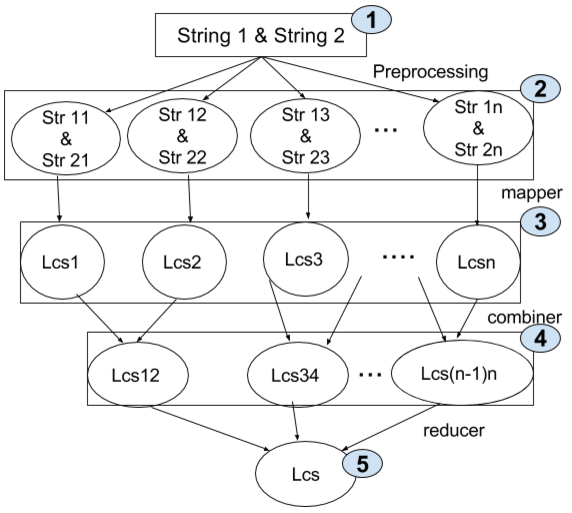
\includegraphics[scale=0.35]{flow-diagram}
\caption{Program Execution Block Diagram}
\label{fig:flow_diagram}
\end{figure}

The basic block diagram of the program execution is shown in figure \ref{fig:flow_diagram} and explained below.

\begin{enumerate}
\item Input string. It is converted to hadoop input by splitting it in multiple parts. The process of splitting given string to the multiple parts is known as preprocessing.
\item Splitted String. It is now feed to mapper to calculated the lcs of each small chunk.
\item Preliminary lcs. This is output of the mapper. Now it is feed to combiner which used parallel algorithm to find intermediate lcs. 
\item Intermediate lcs. This is output of the combiner. In reducer, Multiple intermediate lcs are merged together using parallel algorithm recursively until final lcs is generated. 
\item Final lcs. output of the reducer.
\end{enumerate}

\subsection{Computing LCS using Row-wise processing Technique}
The row-wise processing is inherited from the traditional approach for filling the dynamic programming table. 
However, this time, we concentrate only on those table entries which correspond to a match. 
Each dominant match defines a new corner to a contour line. 
To maintain the columns where all contour lines cross the current row, we use the array $MinYPrefix[1..p]$, 
where $MinYPrefix[l]$ gives the Y-index where the l'th contour line is located. As the name of the array 
suggests, the value of $MinYPrefix[l]$ may be regarded as a cursor, which indicates the minimum 
length prefix of Y that is needed to produce a common subsequence of length l with the first i elements of X. 
Value p denotes $r(X[1..i], Y[1..n])$, that is, the number of contour lines crossing row i. 
Initially, the values of MinYPrefix are initialized to 'undefined'.


\begin{table}[h]
\caption{Table for computing lcs}
\begin{center}
    \begin{tabular}{| c | c | c | c | c | c | c | c | }
    \hline
    \multirow{2}{*}{Row} & \multicolumn{7}{ |c| }{MinYPrefix} \\ \cline{2-8}
     & 0 & 1 & 2 & 3 & 4 & 5 & 6 \\ \hline
    0 & 0 &   & & & & & \\ \hline
    1 & 0 & 3 & & & & & \\ \hline
    2 & 0 & 2 & 5 & & & &\\ \hline 
    3 & 0 & 1 & 4 &  & & & \\ \hline 
    4 & 0 & 1 & 4 &  &  & & \\ \hline 
    5 & 0 & 1 & 2 & 5 &  &  & \\ \hline
    6 & 0 & 1 & 2 & 5 & 8 &  &  \\ \hline
    \end{tabular}
    \end{center}
\label{tab:lcs}
\end{table}

Given the example strings X=abcdbb and Y=cbacbaaba, the values of the array change as follows (undefined values are represented by n+1; the leftmost entry acts as sentinel and is set to zero):

To maintain the MinYPrefix values when moving from row to row, we need the following result.

Update rule: Let us assume that we are processing row i. For each open interval $MinYPrefix[l]..MinYPrefix[l+1]$, (l=0..r), find the matches (i,j) which fall into it (i.e. matches for which the j value is in the interval). The right boundary of the interval is kept unchanged, of no such match exists. Otherwise, it is updated to the smallest such j value (leftmost match in the interval). Note that the updates are simultaneous.

For example, when moving from row 2 to row 3 in the above example, we notice that $X[3] = Y[4]$ and $MinYPrefix[1] < 4 < MinYPrefix[2]$, so we update $MinYPrefix[2]$ to 4. The general scheme for advancing in the dynamic programming table is the following
\\
.\hspace{0.5cm} \textbf{begin}\\
(1) \hspace{0.5cm} \textbf{for} i:= 1 \textbf{to} m \textbf{do} MinYPrefix[i] := n+1; \\
(2) \hspace{0.5cm} MinYPrefix[0] := 0; r := 0; \\
(3) \hspace{0.5cm} \textbf{for} i := 1 \textbf{to} m \textbf{do} \\
. \hspace{1.4cm} /*Update the array values for row i. */\\
(4) \hspace{1.0cm} \textbf{for} j := 0 \textbf{to} r \textbf{do} \\
(5) \hspace{1.4cm} \textbf{if} range[MinYPrefix[j]+1..MinYPrefix[j+1] - 1] \\.\hspace{2.5cm} contains matches \textbf{then}\\
(6) \hspace{1.5cm} \textbf{begin} MinYPrefix[j+1] \\ .\hspace{2.0cm}:= min \{ l or (i, l) is a match in this range\};\\
(7) \hspace{1.6cm} \textbf{if} j = r \textbf{then} r := r+1;\\
  .\hspace{1.6cm}  \textbf{end}; \\
    .\hspace{1.1cm}\textbf{return} r;\\
    .\hspace{0.6cm} \textbf{end}; \\


\subsection{Parallel Implementation}
A scalable parallel version of the LCS algorithm, proposed in \cite{bastola}, is outlined in figure \ref{fig:parallel}. First, each string is divided across the processors and the LCS of the substrings in each processor (LCS1 and LCS2) are computed. Then the portions of strings (grey areas) that were beyond the first and last positions in the LCS are interchange and LCS for these previously unused strings is computed. Finally, the respective portions are combined to obtain the complete LCS.\\

\begin{figure}[h]
\centering
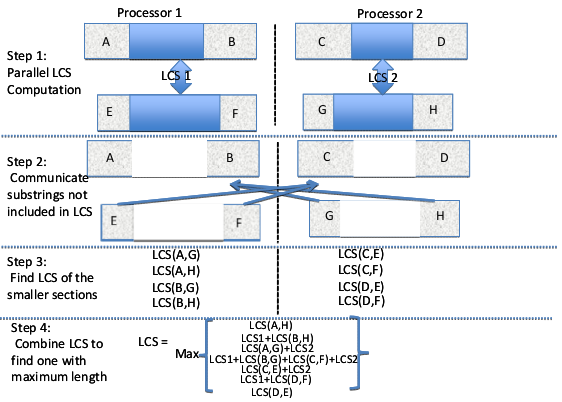
\includegraphics[scale=0.35]{parallel}
\caption{A Schematic Diagram of the Parallel LCS Algorithm}
\label{fig:parallel}
\end{figure}

% needed in second column of first page if using \IEEEpubid
%\IEEEpubidadjcol

% An example of a floating figure using the graphicx package.
% Note that \label must occur AFTER (or within) \caption.
% For figures, \caption should occur after the \includegraphics.
% Note that IEEEtran v1.7 and later has special internal code that
% is designed to preserve the operation of \label within \caption
% even when the captionsoff option is in effect. However, because
% of issues like this, it may be the safest practice to put all your
% \label just after \caption rather than within \caption{}.
%
% Reminder: the "draftcls" or "draftclsnofoot", not "draft", class
% option should be used if it is desired that the figures are to be
% displayed while in draft mode.
%
%\begin{figure}[!t]
%\centering
%\includegraphics[width=2.5in]{myfigure}
% where an .eps filename suffix will be assumed under latex, 
% and a .pdf suffix will be assumed for pdflatex; or what has been declared
% via \DeclareGraphicsExtensions.
%\caption{Simulation Results}
%\label{fig_sim}
%\end{figure}

% Note that IEEE typically puts floats only at the top, even when this
% results in a large percentage of a column being occupied by floats.


% An example of a double column floating figure using two subfigures.
% (The subfig.sty package must be loaded for this to work.)
% The subfigure \label commands are set within each subfloat command, the
% \label for the overall figure must come after \caption.
% \hfil must be used as a separator to get equal spacing.
% The subfigure.sty package works much the same way, except \subfigure is
% used instead of \subfloat.
%
%\begin{figure*}[!t]
%\centerline{\subfloat[Case I]\includegraphics[width=2.5in]{subfigcase1}%
%\label{fig_first_case}}
%\hfil
%\subfloat[Case II]{\includegraphics[width=2.5in]{subfigcase2}%
%\label{fig_second_case}}}
%\caption{Simulation results}
%\label{fig_sim}
%\end{figure*}
%
% Note that often IEEE papers with subfigures do not employ subfigure
% captions (using the optional argument to \subfloat), but instead will
% reference/describe all of them (a), (b), etc., within the main caption.


% An example of a floating table. Note that, for IEEE style tables, the 
% \caption command should come BEFORE the table. Table text will default to
% \footnotesize as IEEE normally uses this smaller font for tables.
% The \label must come after \caption as always.
%
%\begin{table}[!t]
%% increase table row spacing, adjust to taste
%\renewcommand{\arraystretch}{1.3}
% if using array.sty, it might be a good idea to tweak the value of
% \extrarowheight as needed to properly center the text within the cells
%\caption{An Example of a Table}
%\label{table_example}
%\centering
%% Some packages, such as MDW tools, offer better commands for making tables
%% than the plain LaTeX2e tabular which is used here.
%\begin{tabular}{|c||c|}
%\hline
%One & Two\\
%\hline
%Three & Four\\
%\hline
%\end{tabular}
%\end{table}


% Note that IEEE does not put floats in the very first column - or typically
% anywhere on the first page for that matter. Also, in-text middle ("here")
% positioning is not used. Most IEEE journals use top floats exclusively.
% Note that, LaTeX2e, unlike IEEE journals, places footnotes above bottom
% floats. This can be corrected via the \fnbelowfloat command of the
% stfloats package.



\section{Result and Discussion}
In implementing algorithm, the program is divided into 4 steps, that are 1. Preliminary Step, 2. Mapper Step, 3. Combiner Step and 4. Reducer Step. The output of the one step is fed to the consequent next step as input and final step output is received as program output. We used json format as intermediate data format. The example of input data and output data format for each of the processes is as follow.

\begin{enumerate}
    \item Preliminary Step

Here, we have to calculated the lcs of strings str1 and str2. First, we take partition size as 15 and divide each string as a 15 char substring and keep the string sequence order. This work is done in Preliminary Step.

\textbf{Input}\\
str1=ABCBDABATCGACGATCGGGGTTCTTCACCACG\\
 GGGTTCTTCACCAGAGTTATCT \\
str2=BDCABACTCAGGCACCGCAGTGACAAAAGTCG\\CAGTGACAAAAGTCAGGACGGC\\
Partition size: 15\\

\textbf{Output}\\
1   {"a": "ABCBDABATCGACGA", "index": 0, "b": "BDCABACTCAGGCAC"}\\
2  {"a": "TCGGGGTTCTTCACC", "index": 1, "b": "CGCAGTGACAAAAGT"}\\
3  {"a": "ACGGGGTTCTTCACC", "index": 2, "b": "CGCAGTGACAAAAGT"}\\
4  {"a": "AGAGTTATCT", "index": 3, "b": "CAGGACGGC"}\\

\item Mapper Step\\
The preprocess string is fed to mapper. Mapper Process is responsible to find lcs of the small substring of str1 and str2. Along with lcs, it also calculate A, B, E, F and its index which is helpful to calculate combine lcs in upcoming step.

\textbf{Input}\\
Mapper1:  {'a': 'ABCBDABATCGACGA', 'index': 0, 'b': 'BDCABACTCAGGCAC'}\\
Mapper2:  {'a': 'TCGGGGTTCTTCACC', 'index': 1, 'b': 'CGCAGTGACAAAAGT'}\\
Mapper3:  {'a': 'ACGGGGTTCTTCACC', 'index': 2, 'b': 'CGCAGTGACAAAAGT'}\\
Mapper4:  {'a': 'AGAGTTATCT', 'index': 3, 'b': 'CAGGACGGC'}\\

\item Combiner Step\\
Combiner step combine the output of the 2 mappers within the system to give intermediate output.

\textbf{Input}\\
Combiner1: \\
Key: 0  \\
Value: [[0, {'A': 'ABC', 'a': 0, 'B': u'', 'E': u'', 'lcs': 'BDABATCAGA', 'F': 'C', 's2': 'BDCABACTCAGGCAC', 's1': 'ABCBDABATCGACGA', 'f': 15, 'b': 15, 'e': 0}], [1, {'A': 'T', 'a': 0, 'B': u'', 'E': u'', 'lcs': 'CGGTAC', 'F': 'AAAAGT', 's2': 'CGCAGTGACAAAAGT', 's1': 'TCGGGGTTCTTCACC', 'f': 15, 'b': 15, 'e': 0}]]\\ \\
Combiner2: \\
Key: 1  \\
value:  [[2, {'A': 'A', 'a': 0, 'B': u'', 'E': u'', 'lcs': 'CGGTAC', 'F': 'AAAAGT', 's2': 'CGCAGTGACAAAAGT', 's1': 'ACGGGGTTCTTCACC', 'f': 15, 'b': 15, 'e': 0}], [3, {'A': u'', 'a': 0, 'B': u'', 'E': 'C', 'lcs': 'AGGAC', 'F': 'GGC', 's2': 'CAGGACGGC', 's1': 'AGAGTTATCT', 'f': 9, 'b': 10, 'e': 0}]]\\

\item Reducer Process\\
Finally, reducer step reduces the intermediate output from all combiner to one final lcs. 

\textbf{Input:}\\
Key:  lcs  \\
value:  [[0, {'a': 0, 'A': u'', 'b': 30, 'e': 0, 'lcs': 'BDABATCAGACCGGTAC', 'f': 30, 's2': 'BDCABACTCAGGCACCGCAGTGACAAAAGT', 's1': 'ABCBDABATCGACGATCGGGGTTCTTCACC', 'F': u'', 'B': u'', 'E': u''}], [1, {'a': 0, 'A': u'', 'b': 25, 'e': 0, 'lcs': 'CGGTACAGGAC', 'f': 24, 's2': 'CGCAGTGACAAAAGTCAGGACGGC', 's1': 'ACGGGGTTCTTCACCAGAGTTATCT', 'F': u'', 'B': u'', 'E': u''}]]\\ \\
\textbf{Output:}\\
{"length": 28, "lcs": "BDABATCAGACCGGTACCGGTACAGGAC"}\\
\end{enumerate}


\subsection{Complexity Analysis}
The time complexity of core LCS computing algorithm is $O(\text{\textbar} M\text{\textbar} log(n))$ where $\text{\textbar}M\text{\textbar}$ denotes the number of all matches. The space complexity of the algorithm is $O(n^2)$.
\\
\subsection{Run Time of Algorithm}
Performance is measured by running this algorithm for two input sequences. Below are the results for the time taken with single node. The configuration is Intel Core i5 CPU and 8GB of RAM. The linux version is ubuntu 14.04. Two input sequences are run  for 10 times and average time is computed. The time taken by this algorithm is listed below. 
\\
String with length : 55 and 54 with lcs of length 28, per process length 15\\
1. 144.27113533  ms\\
2. 134.327173233  ms\\
3. 153.401851654  ms\\
4. 148.401021957  ms\\
5. 153.903961182  ms\\
6. 130.937099457  ms\\
7. 145.685195923  ms\\
8. 140.298128128  ms\\
9. 145.020008087  ms\\
10. 184.189081192  ms\\
average:  148.043465614\\

string with length 17990 and 17990 with lcs of length 17984 and per process length of

\begin{table}[h]
\caption{Output time comparison with different per process length of the string}
\begin{center}
    \begin{tabular}{| c | c | c | c | c| }
    \hline
\multirow{2}{*}{S.N.} & \multicolumn{4}{|c|}{Per Process Length} \\ \cline{2-5}
& 1500 & 500  & 100 & 50 \\ \hline
1 & 188051 ms & 23204 ms & 2010 ms & 940 ms \\ \hline
2 & 190373 ms & 22622 ms & 1951 ms & 961 ms \\ \hline
3 & 204989 ms & 22590 ms & 2030 ms & 919 ms  \\ \hline
4 & 197026 ms & 22865 ms & 2024 ms & 958 ms  \\ \hline
5 & 200978 ms & 22701 ms & 2093 ms & 961 ms  \\ \hline
6 & 191984 ms & 23751 ms & 2012 ms & 943 ms \\ \hline
7 & 197794 ms & 22773 ms & 1960 ms &  961 ms  \\ \hline
8 & 195714 ms & 22595 ms & 1981 ms & 927 ms  \\ \hline
9 & 206259 ms & 38038 ms & 2057 ms & 909 ms \\ \hline
10 & 204288 ms & 24651 ms & 2021 ms & 949 ms \\ \hline
average & 197746 ms & 24579 ms & 2014 ms & 943 ms \\ \hline
\end{tabular}
\end{center}
\label{tab:lcs}
\end{table}

It is seen that computation time reduced tremendously with smaller per process string length. Though time reduced tremendously with small number of per process string length, the output length of the LCS string also get reduced. We need to make trade-off between time and quality (length of the lcs). 


\subsection{Conclusion}
A basic model for MapReduce based parallel algorithm for gene sequence comparison has been implemented. Although there are few parallel algorithms for LCS computation, they are not reliable as the MapReduce based solution in the context of fault tolerance and concurrency control. This MapReduce based model handles all the different aspects of distributed computing from load balancing to synchronization automatically. The algorithm is highly scalable. Hence, the large number of gene data can be processed at short period if we use the large number of nodes created from commodity computers.

\subsection{Limitation}
The parallel algorithm might not give accurate result if multiple starting and ending point are possible for the same length of the lcs substring between two strings. This is because, with different value of starting and ending sequence, we have different A, B, E, F. So there is always a possibility of not having longest subsequence.

\subsection{Further Enhancement}
There is special case where this algorithm don’t work which is listed in limitation. So we can optimize algorithm to overcome the listed problem. Also we can enhance it to compare the runtime between different distributed platform like Apache Spark, Google dataflow and Hadoop cascading.

\begin{thebibliography}{9}
\addcontentsline{toc}{section}{References}

\bibitem{bastola}
S. Bhowmick, M. Shafiullah, H. Rai, and D. Bastola, “A Parallel Non-Alignment Based Approach to Efficient Sequence Comparison using Longest Common Subsequences,” J. Phys.: Conf. Ser. Journal of Physics: Conference Series, vol. 256, p. 012012, Jan. 2010.

\bibitem{needleman}
S. B. Needleman and C. D. Wunsch, “A general method applicable to the search for similarities in the amino acid sequence of two proteins,”Journal of Molecular Biology, vol. 48, no. 3, pp. 443–453, 1970.

\bibitem{waterman}
T. F. Smith and M. S. Waterman, “Comparison of biosequences,” Advances in Applied Mathematics, vol. 2, no. 4, pp. 482–489, 1981.

\bibitem{hirschberg}
D.S. Hirschberg, A linear space algorithm for computing maximal common subsequences, Comm. Assoc. Comput. Mach., 18:6, 341–343, 1975.

\bibitem{hunt}
J.W Hunt, and T.G Szymanski. "A Fast Algorithm for Computing Longest Common Subsequences". Comm. ACM, vol.20 no.5; 350-353. 1977.

\bibitem{chen}
Y. Chen, A. Wan and W. Liu, "A fast Parallel Algorithm for finding the Longest Common Subsequence of multiple biosequences" , BMC Bioinformatics 7 (suppl 4), 2006

\bibitem{eswaran}
S. Eswaran and S.P. RajaGopalan, "An Efficient Fast Pruned Parallel Algorithm for finding LCS in Biosequences", Anale Seria Informatica. Vol. VIII fasc.1, 2010.

\bibitem{dhraief}
A. Dhraief, R. Issaoui and A. Belghith, "Parallel Computing the Longest Common Subsequence (LCS) on GPUs: Efficiency and Language Suitability", INFOCOMP 2011: The First International Conference on Advanced Communications and Computation, 2011

\bibitem{bohora}
J. Bohara, S.R. Joshi, "A MapReduce Based Parallel Algorithm for Finding Longest Common Subsequence in Biosequences", IOE Graduate Conference Journal, 2013

\end{thebibliography}


% if have a single appendix:
%\appendix[Proof of the Zonklar Equations]
% or
%\appendix  % for no appendix heading
% do not use \section anymore after \appendix, only \section*
% is possibly needed

% use appendices with more than one appendix
% then use \section to start each appendix
% you must declare a \section before using any
% \subsection or using \label (\appendices by itself
% starts a section numbered zero.)
%


% trigger a \newpage just before the given reference
% number - used to balance the columns on the last page
% adjust value as needed - may need to be readjusted if
% the document is modified later
%\IEEEtriggeratref{8}
% The "triggered" command can be changed if desired:
%\IEEEtriggercmd{\enlargethispage{-5in}}

% references section

% can use a bibliography generated by BibTeX as a .bbl file
% BibTeX documentation can be easily obtained at:
% http://www.ctan.org/tex-archive/biblio/bibtex/contrib/doc/
% The IEEEtran BibTeX style support page is at:
% http://www.michaelshell.org/tex/ieeetran/bibtex/
%\bibliographystyle{IEEEtran}
% argument is your BibTeX string definitions and bibliography database(s)
%\bibliography{IEEEabrv,../bib/paper}
%
% <OR> manually copy in the resultant .bbl file
% set second argument of \begin to the number of references
% (used to reserve space for the reference number labels box)

% You can push biographies down or up by placing
% a \vfill before or after them. The appropriate
% use of \vfill depends on what kind of text is
% on the last page and whether or not the columns
% are being equalized.

%\vfill

% Can be used to pull up biographies so that the bottom of the last one
% is flush with the other column.
%\enlargethispage{-5in}

% that's all folks
\end{document}


